\documentclass{article}
\usepackage{graphicx}
\begin{document}
\title{Bolometric Light Curves: Nickel masses for low reddening Type Ia supernovae}
\maketitle
We have observed that the timing of the second maximum in the NIR filters ($YJH$) is strongly dependent on the light curve decline rate, and hence, the peak brightness of the supernova. Since the brightness of the supernova is known to be driven by the amount of Ni synthesized, we investigate the relation between the calculated Nickel masses for a sample of 'normal' SNIa

Arnett's rule (Arnett 1982) states that the luminosity of an SNIa at peak is equal to the instantaneous energy deposition rate from the radioactive decay of $^{56}$Ni. Using this equivalence, we can calculate the amount of Nickel produced by a supernova from measuring the peak of the bolometric light curve. This has been done recently for a sample of SNfactory supernovae in Scalzo et al. [2014]. The details of the radioactive decay are presented in Nadyozhin 1994. 





\section{The sample}
For the initial part of the study, we constrain the sample to objects with a measured $t_2$ and multi-band coverage to obtain a (pseudo-)bolometric light curve. Previous studies to calculate Nickel masses from the bolometric peak have used extinction corrections for the optical light curves. In order to minimize the error from the extinction and any effects from the presumed extinction law, we only select objects with $E(B-V)_{host}<$0.1. From the CSP dataset, this leaves us with 17 objects for which we have bolometric light curves, extending to late times.  


\section{Method}
Bolometric light curves were calculated from multi-band photometry. The magnitudes were corrected 
for reddening using a CCM reddening law for each filter ({\bf check, however, we are trying to 
circumvent this by using a low reddening sample}). 
Using zero-points in the given filters, the magnitudes were converted to fluxes. 
The resulting light curve, in ergs/$cm^2$/s  was converted into an absolute bolometric light curve 
by using the distances of the SN from the host galaxy redshift.  
{\bf describe Stephane's routine in more detail here}

\section{Analysis}
$t_2$ measurements are described in paper draft

The bolometric light curves were interpolated using a cubic spline. In order to get an $L_{Bol}(max)$ we required sampling in the individual bands at pre-maximum epochs. The errors on the peak were calculated from the errors in the fluxes of the bolometric maximum.  

In order to obtain the Nickel mass from the bolometric peak luminosity, we interpolate the values obtained by the DDC models of Blondin et al. [2013]. For objects without NIR coverage near maximum, we use the interpolated values for the BVRI filters only.  

The resulting Nickel mass estimates for our sample are presented in Table~\ref{tab:mni}.
\begin{table*}
\caption{$L_{max}$ measurements for low reddening SNIa with a measured $t_2$. }

\begin{center}
\begin{tabular}{llccccrrr}
\hline
SN  & $L_{max}(\cdot e^{43} erg s^{-1})$ & $e_{L}$  & $M_{Ni}-Arn (M_{\odot})$  & $M_{Ni}-Arn (M_{\odot})$ (fixed rise)  & $M_{Ni}-DDC (M_{\odot})$\\% & $E(B-V)_{MW}$ & u-band lum \\
\hline
%SN2001ba & 1.18 & 0.15 & 0.58 & 0.59 & 	0.57 \\
SN2002dj & 1.25 & 0.26 & 0.59 & 0.63 & 0.61 \\
SN2002fk & 1.42 & 0.23 & 0.68 & 0.71 & 0.76 \\
SN2005M & 1.37 & 0.08 & 0.70 & 0.69 & 0.71 \\
SN2005am & 1.1 & 0.2 & 0.47 & 0.55 & 0.52 \\
SN2005el & 0.91	& 0.11 & 0.40 & 0.46   & 0.44 	\\	
SN2005eq & 1.32 & 0.2 & 0.67 & 0.66 & 0.67 \\
SN2005hc & 1.36 & 0.2 & 0.69 & 0.68 & 0.71 \\
SN2005iq & 1.07 & 0.11 & 0.48 & 0.54 & 0.51 \\
SN2005ki & 1.03 & 0.27 & 0.45 & 0.51 & 0.49 \\
SN2006bh & 0.86 & 0.15 & 0.37 & 0.43 & 0.40 \\
SN2007bd & 1.22 & 0.13 & 0.55	  & 0.61 & 0.59	\\
SN2007on & 0.6 & 0.09 & 0.24 & 0.30 & 0.28 \\
SN2008R & 0.53 & 0.1 & 0.21 & 0.26 & 0.25 \\
SN2008bc & 1.24 & 0.19 & 0.60 & 0.62 & 0.63 \\
SN2008gp & 1.29 & 0.14 & 0.62 & 0.65 & 0.64 \\
SN2008hv & 1.08 & 0.13 & 0.48 & 0.54 & 0.52 \\
SN2008ia & 1.13 & 0.14 & 0.50 & 0.57 & 0.55 \\
SN2011fe & 1.1 & 0.15 & 0.50 & 0.55 & 0.52 \\
\hline
\end{tabular}
\label{tab:mni}
\end{center}
\end{table*}

\begin{figure}
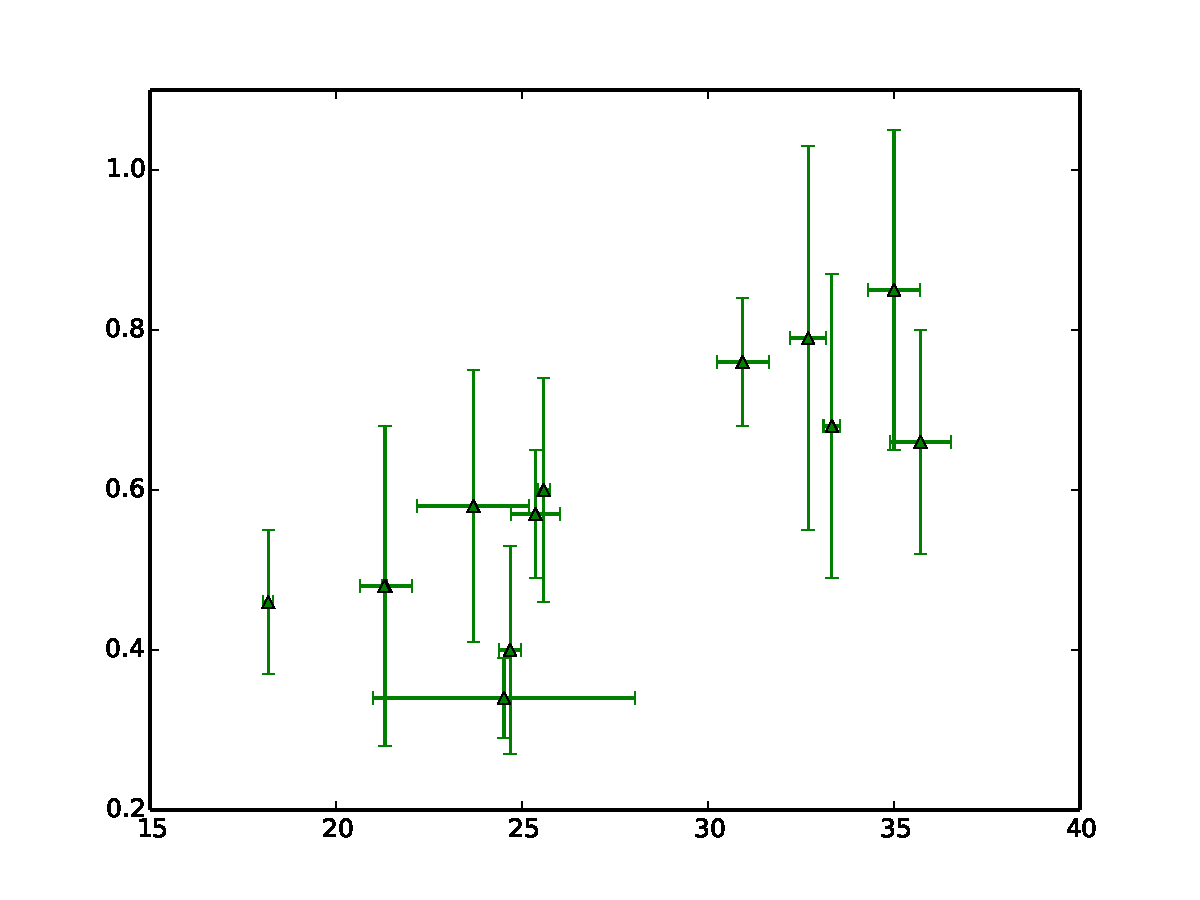
\includegraphics[width=.6\textwidth, trim= 0 30 0 30]{../../bol_ni_ej/ni_t2.pdf}
\caption{The $^{56}$Ni mass plotted against the timing of the secomd maximum. A correlation with $r$=0.84 is observed}
\label{fig:t2_mni}
\end{figure}

From figure ~\ref{fig:t2_mni}, we conclude that there is a strong correlation between the amount of Ni produced in a SNIa and the timing of the second maximum ({\bf $J$ band currently, make three subplots}) The $p$-value for the probability that the correlation is a chance event is 1e-5. 



\section{Test Case SNae}
Using the correlation derived above, we want to estimate the Ni masses of heavily reddened SNae. The first test case si the nearby SN 2014J in M82 with an EBV of 1.3. Current attempts to use the bolometric light curve depend on the $A_v$ value used and vary by a factor of 2 (0.37 $M_{\odot}$ in Margutti+2014, compared to 0.77 in Goobar+2014)

The proximity of SN2014J, however, has allowed for the first $\gamma$ ray Co line detection in an SNIa (Churazov+ 2014). the authors, using a line photon escape fractino from the models, deduce an Ni mass of 0.62  $\pm$ 0.13 $M_{\odot}$.

Using the best fit relation for the sample defined above , {\bf add equation. currently giving compiling issues} we obtain $M_{Ni}$ of 0.61 $\pm$ 0.23 $M_{\odot}$  for a $t_2$ of 28.7 $\pm$ 5.7 days. 
%\begin{equation}
%\label{eq:ni}
%$M_{Ni}$=0.022*$t_2$-0.0257
%\end{equation}

This uncertainty in $M_{Ni}$ can be reduced with a more precise estimate of $t_2$

For SN2006X, which has a measured $t_2$ of 28.19 $\pm$ 0.5, we get an $M_{Ni}$ of 0.6 $\pm$ 0.13 $M_{\odot}$. 

\section{Late Decline Rates}
For the NIR filters, we observed that the decline rate in $YJH$ is very uniform, suggesting that different SNIa have a very similar structure. However, even at these late times, the SN emits a very small fraction of the total bolometric flux in the NIR. Thus, we look at the bolometric decline rate in order to provide a more robust conclusion about the distribution of the ejecta.

The bolometric light curves are calculated as above. We use the late time data ($+40<t<+90$ days) in log space to calculate a decline rate. We find that the distribution of this decline rate is extremely uniform with a scatter around mean of $\sim$ 0.003 magnitudes per day. This confirms the interpretation from the NIR data that the ejecta structure is very uniform.

Since we have a sample of SNIa with a well-measured boloemtric light curve that extends to late phases, we perform the same analysis of measuring $M|_{55}$, as we did in the NIR bands. The $M|_{55}$(bol) is the absolute flux at +55 days for the (pseudo-)bolometric light curve. We find that this quantity correlates very strongly with the $\Delta m_{15}$ and the $M_{Ni}$ measured from the peak. We can therefore confirm the conclusion from the NIR data that the different objects having similar decline rate are offset by a factor determined by their Nickel masses.
\begin{figure}
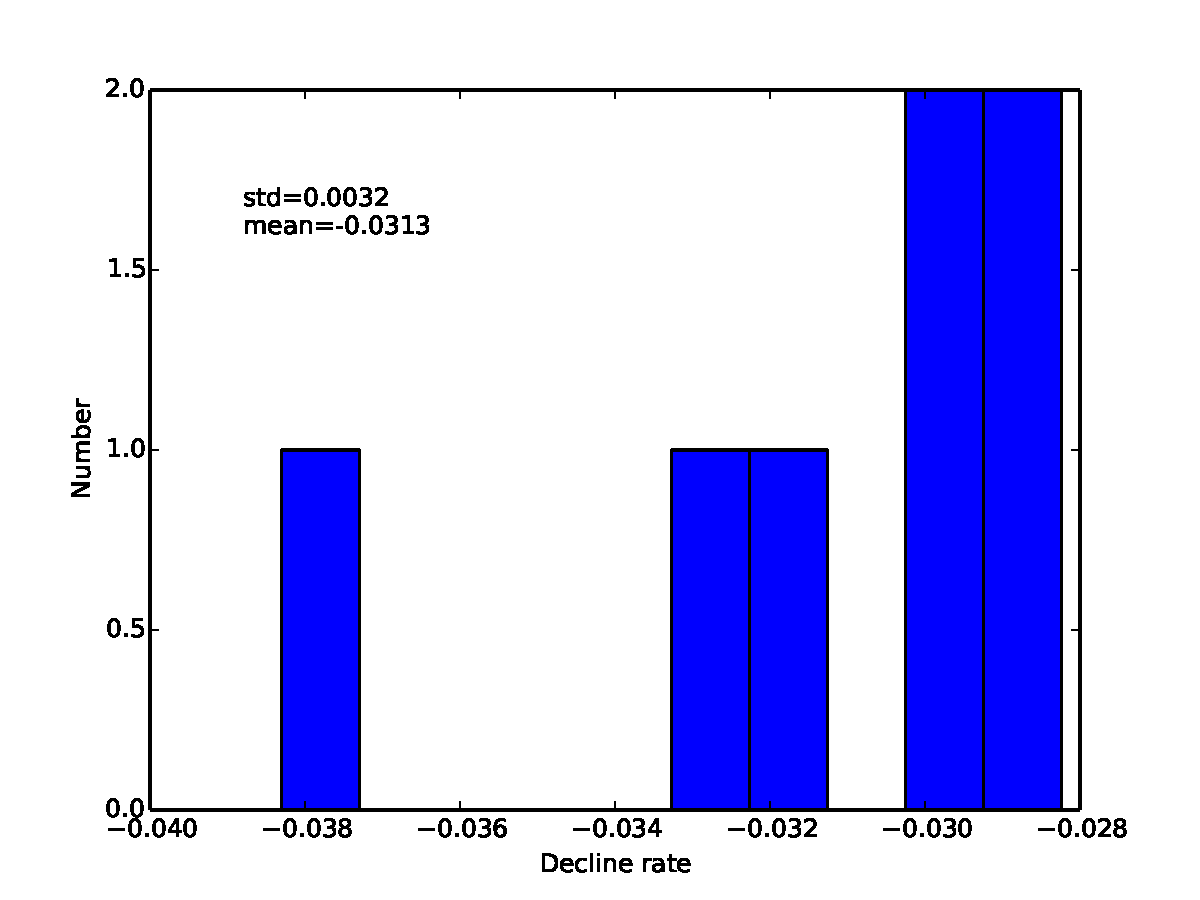
\includegraphics[width=.6\textwidth, trim= 0 30 0 30]{../../bol_ni_ej/Late_decl_distrib.pdf}
\caption{The distribution of late declines in mag/day. The mean and rms scatter is mentioned}
\label{fig:decl}
\end{figure}

\section{Conclusions}
We obtain a strong correlation between the $t_2$ measurements in $YJH$ and the $M_{Ni}$ calculated from the bolometric light curves for the given sample of SNIa. This provides direct evidence for the conlcusions drawn from the correlation between $t_2$ and $\Delta m_{15}$. This indicates that SNIa with more Ni have a slower cooling rate and the ionization transition to FeII happens later, resulting in a later $t_2$.


We have used this relation to get $M_{Ni}$, which, with NIR spectra at late times providing an extinction measurement can be compared to the value from the extinction-corrected light curve

\end{document}

